\chapter{Introduction}
Automatic 3D reconstruction of real objects plays an important role in many applications such as animation, virtual reality, and gaming. A widely used approach to reconstruct an object is by using a 3D laser range scanner. Since range scanners have limited field of view, acquisition of 3D geometry of an object requires taking several scans from different viewpoints. The main difficulty with this method is to combine these scans into a unique surface representing the object. This typically involves two steps. First, all the scans must be transformed into the same coordinate system by a process known as surface registration. Second, the registered scans must be integrated into a single model by a process known as surface integration. In this paper we focus on surface integration, assuming the scans have been acquired and registered in a common coordinate system.

\section{First section}
Existing surface integration methods for range images can be classified into two categories: volume-based and mesh-based. Volume-based methods \cite{Claes:VolM05,Curless:VolM96,Masuda:VolM02,Hoppe:VolM97,Sato:VolM97,Sun:VolM03} convert range images into an intermediate volumetric representation using a signed distance function and extract the final surface using a polygonizing algorithm. These methods can handle objects of arbitrary topology and are considered to be robust with respect to scanning noise, outliers and registration errors. The choice of appropriate voxel size is important for these methods \cite{Claes:VolM05,Curless:VolM96}. If the voxel size is too large, then features smaller than the voxel size are missed and opposite surfaces of a narrow region will be merged. If the voxel size is too small, then in the presence of scanning noise or registration errors, corresponding surfaces will be reconstructed as separate surfaces. It still remains unanswered as to what extent the signed distance function computed on the discretized space is sensitive to the presence of noisy data. It is also not clear how to choose an appropriate voxel size when the input range images have both small features and registration errors. \\

Mesh-based methods \cite{Pito:MeshM96,Rutishauser:MeshM94,Sappa:MeshM00,Soucy:MeshM92,Soucy:MeshM95,Sun:MeshM00,Turk:MeshM94,Zhou:MeshM06} directly integrate range images into a single mesh. These methods do not need an intermediate representation. Hence, they are faster and require less memory compared to volumetric methods. In addition, they are more amenable to data reduction during processing which makes them more feasible for use with very large meshes. Existing methods are, however, sensitive to scanning errors and do not work well on objects with large surface curvature \cite{Curless:VolM96}.

\begin{figure}[t]
    \centering
    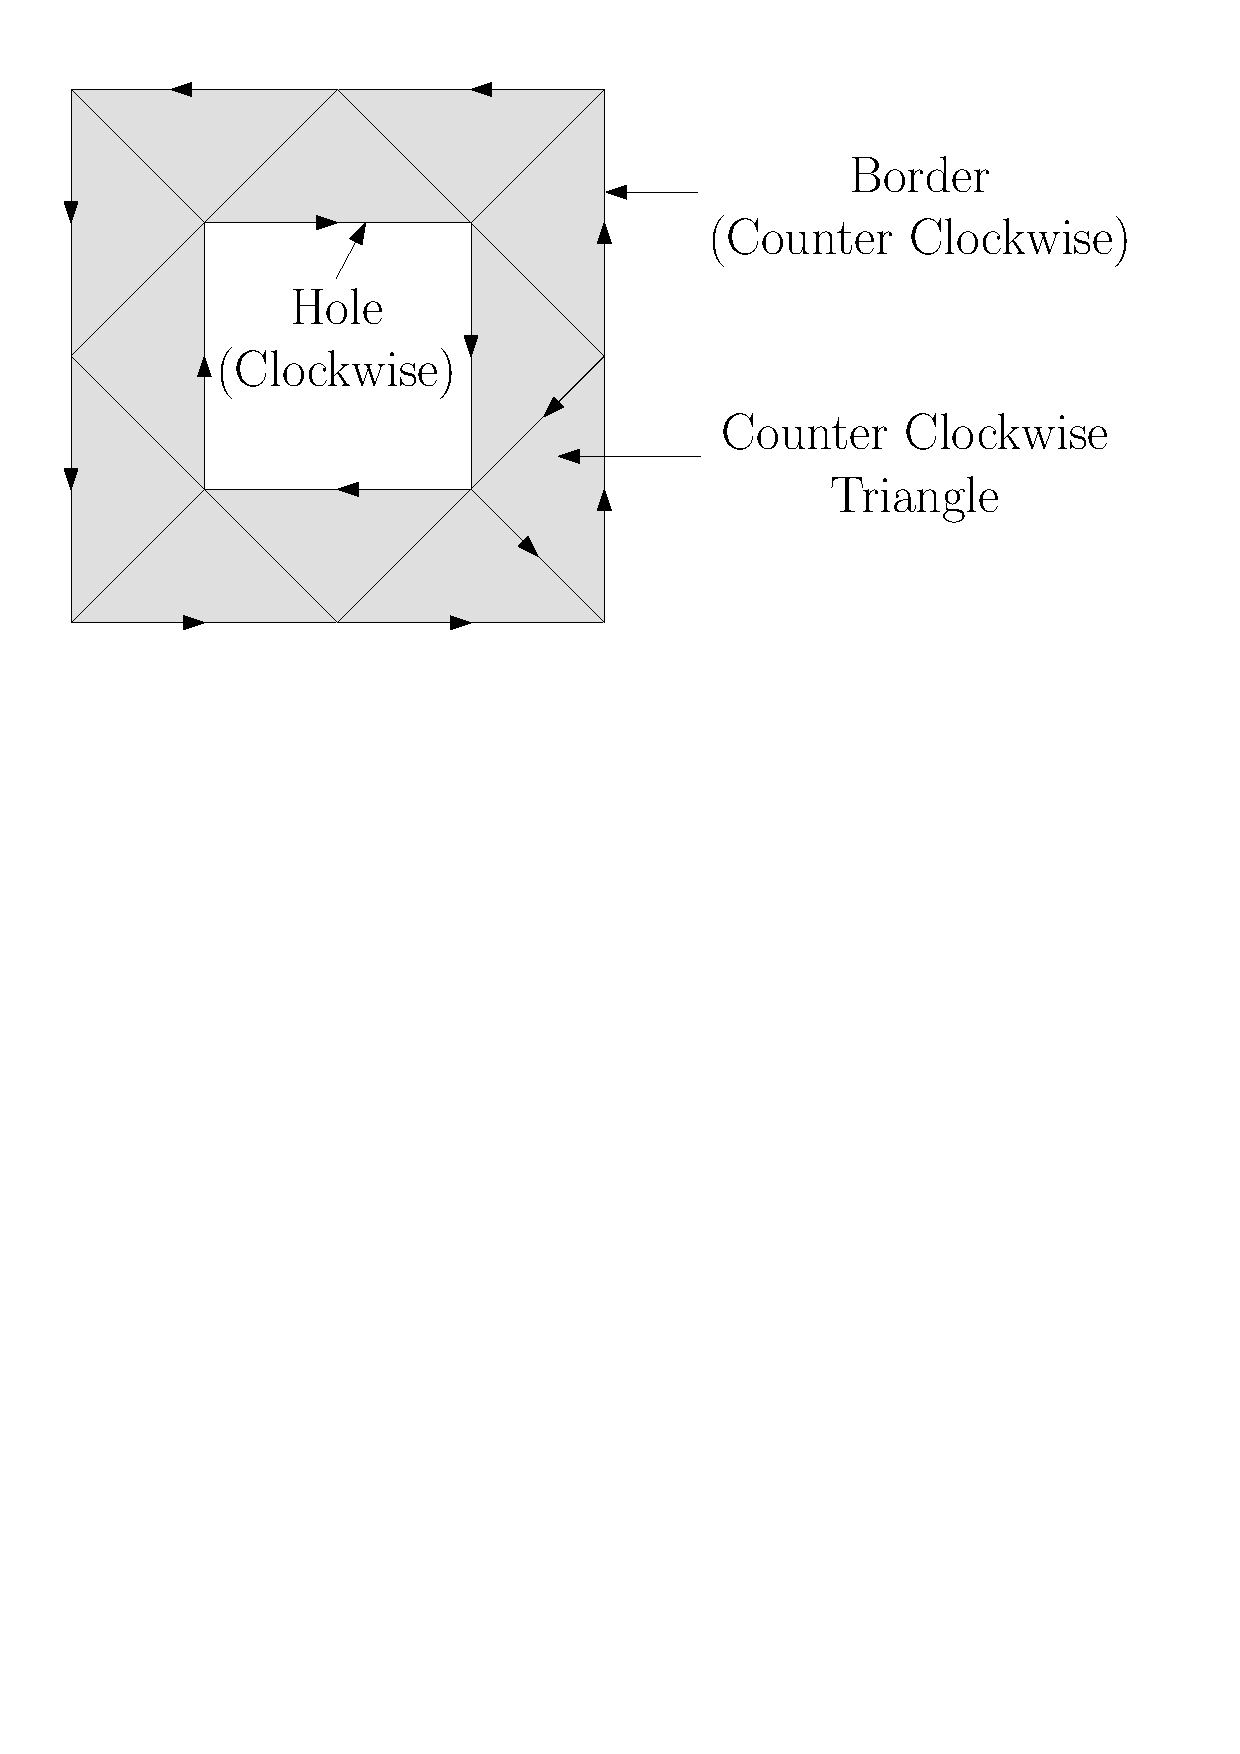
\includegraphics[width=5in]{thesis_SPhd_subfiles/border}
    \caption[Boundary edges]{Boundary edges.}
    \label{fig:Ch1-border}
\end{figure}

\begin{table}[t]
\caption{Statistics for the time taken to merge various models}
\label{table:Ch1-Stats}
\centering
\begin{tabular}{lcccc}
	\toprule
	\textbf{Model} & \textbf{Num. Scans} & \textbf{Input Triangles} & \textbf{Output Triangles} & \textbf{Time Taken (secs)} \\
	\midrule
	Drill & 14 & 102284 & 19152 & 159 \\
	Hello Kitty & 9 & 83627 & 27856 & 237 \\
	Warrior & 10 & 133927 & 34613 & 315 \\
	Doll & 9 & 146080 & 54022 & 479 \\
	Mug & 6 & 114347 & 68129 & 613 \\
	\bottomrule
\end{tabular} 
\end{table}
\let\vect\vec

\begin{SgAlgorithm}[t]
    \SetKwInOut{Input}{Input}
    \SetKwInOut{Output}{Output}
    \SetKwFunction{GenerateAlphaVeins}{GenerateAlphaVeins}
    \SetKwFunction{GenerateUniLeaf}{GenerateUnilobedLeaf}
    \SetKwFunction{IntersectLobes}{IntersectLobes}
    \SetKwFunction{FitBSpline}{FitBSpline}
    \SetKwFunction{GenerateLaminarMargin}{GenerateLaminarMargin}
    \SetKwFunction{Index}{Index}
    \BlankLine
    \Input{Parameters of the leaf model.}
    \Output{Laminar shape $M$ as a triangle mesh.}
    \BlankLine
    $\{\alpha_i\} \leftarrow \GenerateAlphaVeins(s_0^l, s_0^r, \Delta s)$ \;
    $L\leftarrow \GenerateUniLeaf(\theta(B^l), \theta(B^r), \theta(A^l), \theta(A^r), \vect{W}^l, \vect{W}^r)$ \;
    \BlankLine
    \ForEach{$\alpha$-vein $\alpha_i$}
    {%
        $L_i \leftarrow L$ \;
        $L_i \leftarrow T_i\cdot L_i$ \;
    }
    \BlankLine
    \For{$i=1$ \KwTo $n-1$}
    {%
        $\vect{p}^I(v_i) \leftarrow$ \IntersectLobes{$L_i$, $L_{i+1}$} \;
        $\vect{d}(v_i) \leftarrow \dfrac{\vect{d}(\alpha_i) + \vect{d}(\alpha_{i+1})}{2}$ \;
        \If{$p(v)$ or $\theta(v)$ is specified}
        {%
            $\vect{p}(v_i) \leftarrow  \vect{p}^I(v_i) + p(v) l(\alpha_i) \vect{d}(v_i)$ \;
        }
    }
    \BlankLine
    \For{$i=1$ \KwTo $n-1$}
    {%
        \eIf{$p(v)$ or $\theta(v)$ is not specified}
        {%
            $M \leftarrow M \cup \left\{\vect{p}_j \mid j \in L_i \wedge \Index(\vect{q}(\alpha_i), L_i) \leq j \leq \Index(\vect{p}^I(v_i), L_i) \right\}$ \;
          $M \leftarrow M \cup \left\{\vect{p}_j \mid j \in L_{i+1} \wedge \Index(\vect{p}^I(v_i), L_{i+1}) < j \leq \Index(\vect{q}(\alpha_{i+1}), L_{i+1})\right\}$ \;
        }
        {%
           $b_1 \leftarrow \FitBSpline(\vect{q}(\alpha_i), \theta(\vect{q}(\alpha_i)), \vect{W}^l(\alpha_i), \vect{r}(v_i), \theta(v_i))$ \;
            $b_2 \leftarrow \FitBSpline(\vect{r}(v_i), \theta(v_i), \vect{W}^r(\alpha_{i+1}), \vect{q}(\alpha_{i+1}), \theta(\vect{q}(\alpha_{i+1})))$ \;
            Discretize $b_1$ and append the points to $M$ \;
            Discretize $b_2$ and append the points to $M$ \;
        }
    }
    \caption[Laminar shape generation algorithm for multilobed leaves]{Laminar shape generation algorithm for multilobed leaves.}
    \label{algo:Ch6-ShapeGen}
\end{SgAlgorithm}